\section{Schema Hierarchies}
\label{sec:schema_hier}

\begin{figure}
    \centering
    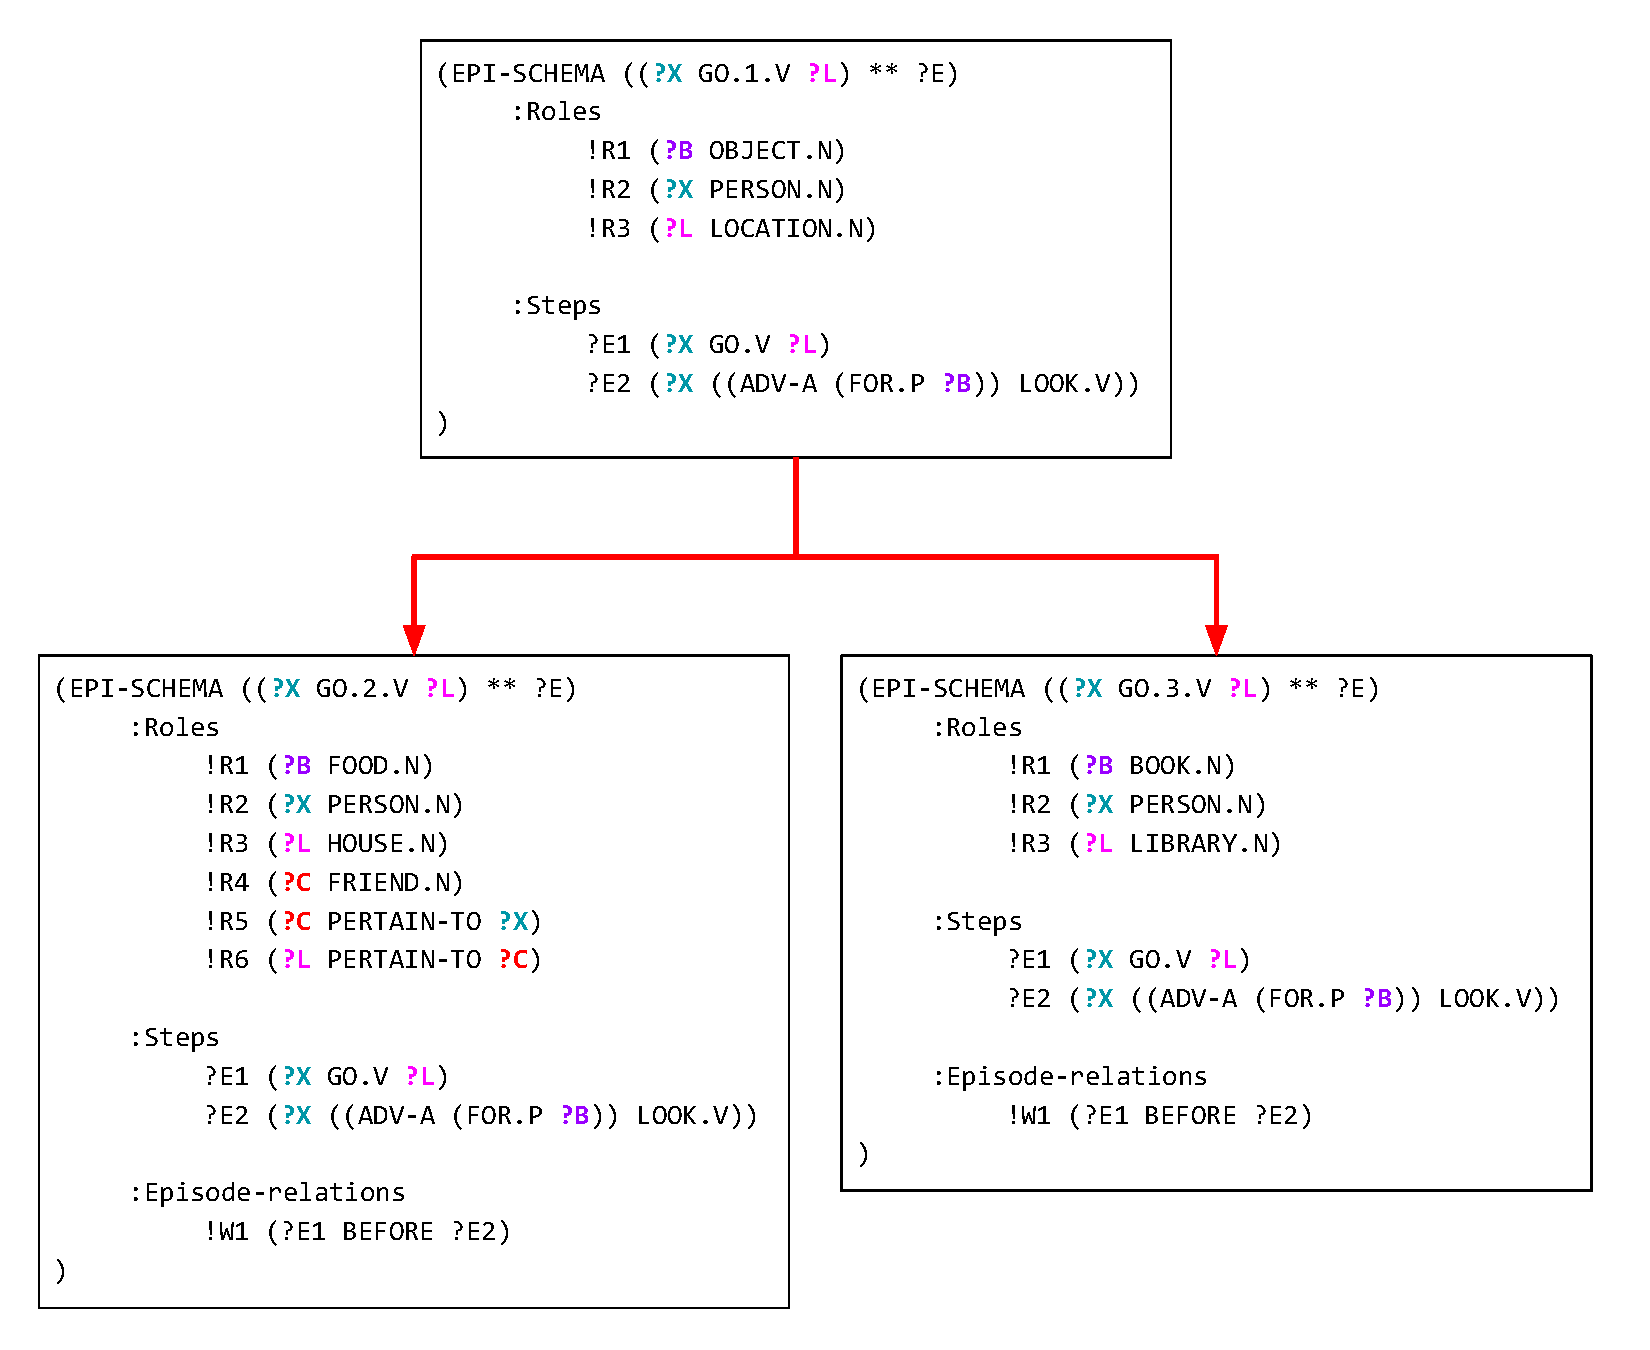
\includegraphics[width=\columnwidth]{CH3_schemas/inheritance}
    \caption{An illustration of the \textbf{taxonomic} hierarchy, in which two \textit{child} schemas inherit the semantics of a shared \textit{parent}.}
    \label{fig:spec_hier}
\end{figure}

\begin{figure}
    \centering
    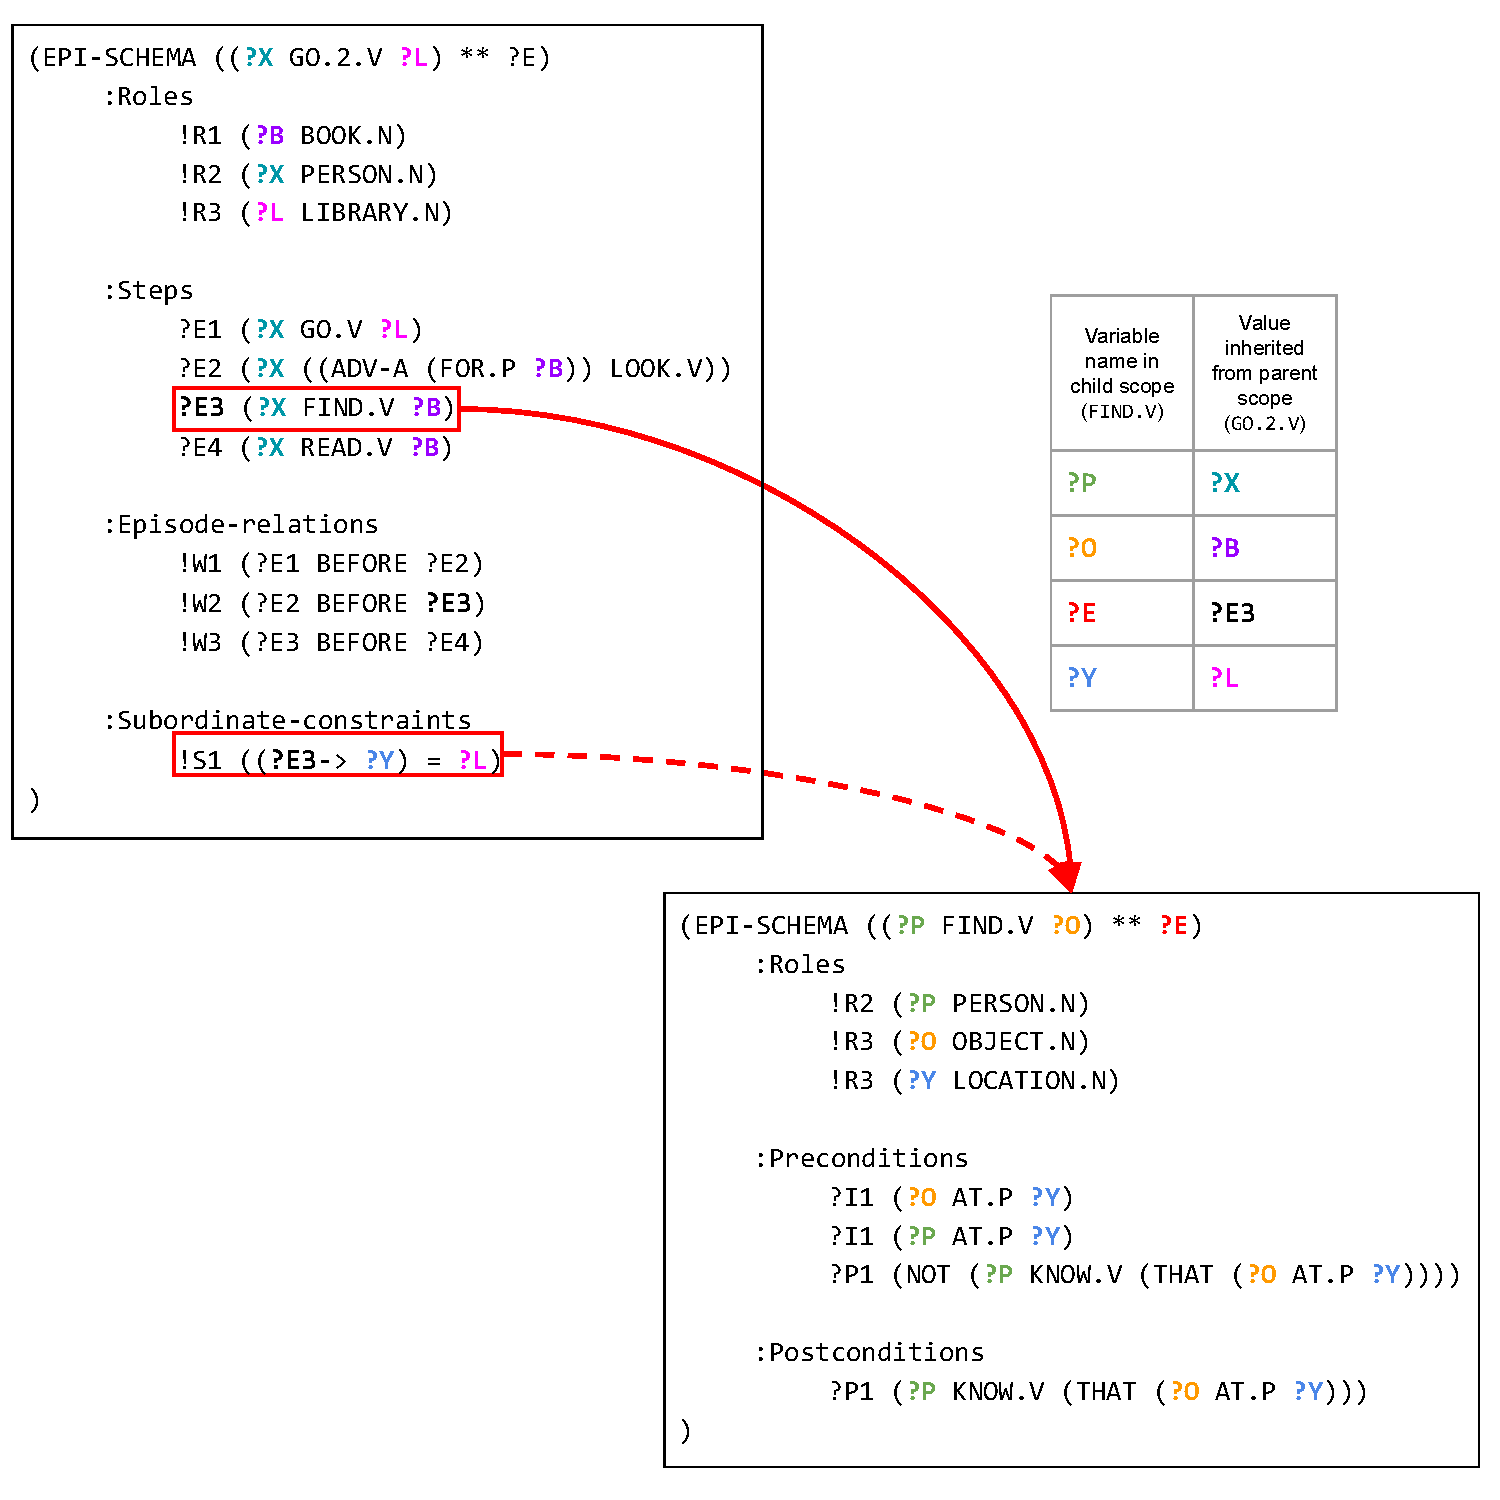
\includegraphics[width=\columnwidth]{CH3_schemas/nesting}
    \caption{An illustration of the \textbf{meronomic} hierarchy, in which a \textit{child} schema is embedded within a \textit{parent}. The child schema \texttt{FIND.V}, shown in the bottom right, is nested within the parent schema \texttt{GO.2.V}, shown in the top left. A table in the upper right shows the new values for the child schema's variables, each inherited from the parent schema.}
    \label{fig:compo_hier}
\end{figure}

EL schemas support two hierarchical organizations of schemas.

In the \textbf{taxonomic} hierarchy, a child schema inherits the semantics of a parent schema, and may then further restrict the set of participants, their types and relationships, and the events; this hierarchy is comparable to an object-oriented ontology based on an IS-A relationship. A taxonomic child schema may add type and relational constraints to its parent schema via the \texttt{:Roles} section, add steps to a parent schema, or replace steps in the parent with taxonomic children of those same steps. An example of a taxonomic schema relationship is given in Figure~\ref{fig:spec_hier}, in which a \textit{person goes somewhere and looks for something} schema, \el{GO.1.V}, is specialized into two child schemas: \el{GO.2.V}, a \textit{go to a friend's house and look for food} schema, and \el{GO.3.V}, a \textit{go to a library and look for a book} schema. A taxonomic parent implicitly shares its variable names with its children, that is, $$\forall v \in dom(\texttt{P}\hspace{-1.5mm}\rightarrow) \hspace{2mm} [ (\texttt{P}\hspace{-1.5mm}\rightarrow v) = (\texttt{C}\hspace{-1.5mm}\rightarrow v)]$$ where \el{P} and \el{C} are the episodes characterized by the parent and child schemas, respectively; $\texttt{P}\hspace{-2mm}\rightarrow$ and $\texttt{C}\hspace{-2mm}\rightarrow$ are their respective variable-binding Skolem functions, as defined in Section~\ref{sec:scoping}; and $dom(\texttt{P}\hspace{-2mm}\rightarrow)$ is the variable domain of the parent's Skolem function. The only exceptions to this rule are the fluent episode IDs $\texttt{?T}n$ in the \texttt{:Inherits-from} section, as these must be locally scoped to allow for relative parent reference. Variable names that are not equal but should be shared with the parent may be constrained explicitly in the \texttt{:Superordinate-constraints} section of the child schema. Because multiple inheritance is allowed, we must address the so-called \textit{diamond problem}, in which a grandchild inherits from two parents, each of which inherits from a shared grandparent; shared variable names as used by the grandchild then become ambiguous, as each of its parents has a different version of the grandparent's, which may be differently constrained. However, as the schema taxonomic hierarchy is generally assumed to be logically \textit{consistent}, we can side-step the diamond problem by concluding that all specialization constraints on shared variables along \textit{any path} of an directed acyclic inheritance graph are \textit{simultaneously true}.

In the \textbf{meronomic} hierarchy, a child schema is \textit{embedded} as a step in a parent schema; it is represented in the parent's \texttt{:Steps} section as its header formula, but can be \textit{expanded} to reveal its full semantics, which include its own steps, participants, and nested schemas.
Because the predicate of the embedded schema's header formula is explicitly associated with one unique schema, the full semantics of the nested schema need not be present in the header; for example, the header formula \el{(?X GO.1.V ?Y)} might correspond to an embedded schema called \el{GO.1.V}, which might specify additional entities and constraints, such as \el{(?Y HOUSE.N)}, \el{(?F FRIEND.N)}, and \el{(?Y PERTAIN-TO ?F)}, to indicate that \el{?X} is going to a friend's house. These predications would all be implicit given the embedded \el{GO.1.V} proposition in the meronomic parent schema.
The scope of the meronomic child schema is inherited from that of the parent, but may have explicit variable bindings specified in the \texttt{:Subordinate-constraints} section, as discussed in Section~\ref{sec:scoping}.

\subsection{Meronomy as Taxonomy}
Under the view that a taxonomic specialization of a schema is the tightening or addition of its constraints, we can, in principle, formulate the meronomic schema hierarchy as a special case of the taxonomic hierarchy. The semantics of meronomic embedding and expansion are simple: when a parent schema $P$ embeds a child schema $C$, all of $C$'s formulas are added to the relevant sections in $P$, with relevant variable replacements being made according to the \texttt{:Subordinate-constraints} and \texttt{:Superordinate-constraints} sections of $P$ and $C$, respectively. This new, ``flattened'' schema, $P^{\prime}$, is semantically equivalent to $P$, but re-formulates the meronomic embedding relationship to $C$ as an addition of constraints to $P$. This allows $P$ to subsume $P^{\prime}$ in the \textit{taxonomic} hierarchy. Put informally, a schema that adds extra events to another schema has an IS-A relationship with that schema. This unification of the meronomic and taxonomic hierarchies can be seen as an extension to the discrimination network model used by IPP (Section~\ref{sec:ipp}), in which edges between S-MOPs indicated \textit{exactly} shared features, rather than the taxonomic and meronomic relations that allow EL schemas to share inexact features.
